\newcommand{\psd}[1]{{\small\sffamily{\color{blue!60}#1}}}


PSD provides mean to time log your solver via \psd{-timelog} flag. What
this will do when you run your solver, on the terminal you will have
information printed on what is the amount of time taken by each step of
your solver. Warning, this will make your solver slower, as this action
involves MPIbarrier routines for correctly timing operation.

An example work flow of 2D solver with timelogging:

\begin{lstlisting}[style=BashInputStyle]
PSD_PreProcess -dimension 2 -problem elastodynamics -dirichletconditions 1 -tractionconditions 1 \
-timediscretization newmark_beta -postprocess uav -timelog
\end{lstlisting}

Once the step above has been performed, we solve the problem using two
MPI processes, with the given mesh file \psd{bar-dynamic.msh}.

\begin{lstlisting}[style=BashInputStyle]
PSD_Solve -np 2 Main.edp -mesh ./../Meshes/2D/bar-dynamic.msh -v 0
\end{lstlisting}

\begin{figure}[h!]
\centering
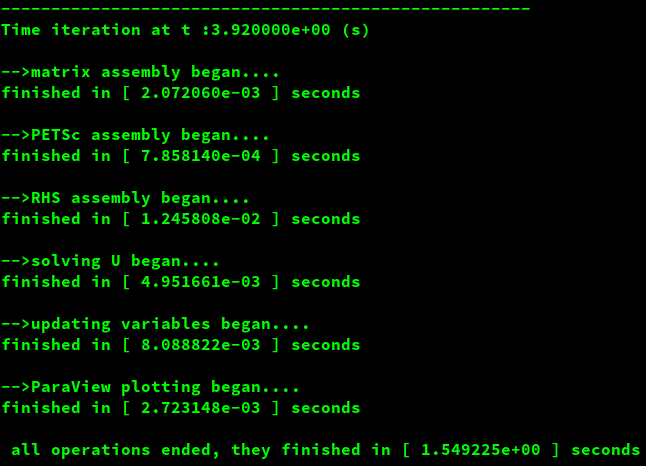
\includegraphics[width=0.4\textwidth]{./Images/ed-time-par.png}
\caption{Time logging output produced for parallel run on 2 processes.\label{time-par-ed}}
\end{figure}

The figure\textasciitilde{}\ref{time-par-ed} shows the time logging
output produced for parallel run on 2 processes using \psd{-timelog}
flag. Similar output is produced for sequential solver of the same
problem shown in figure\textasciitilde{}\ref{time-seq-ed}. Take note of
the speed up, which should be two folds - parallel solver solves the
full problem in half the time (1.5 sec) than that of sequential solver
(3.3 sec). This is due to the fact we used 2 MPI processes.

Also take note of timings produced for different operations of the
solver. Note that in figures\textasciitilde{}\ref{time-par-ed},
\ref{time-seq-ed}, we only see the final time step of the solved
problem.

\begin{figure}[h!]
\centering
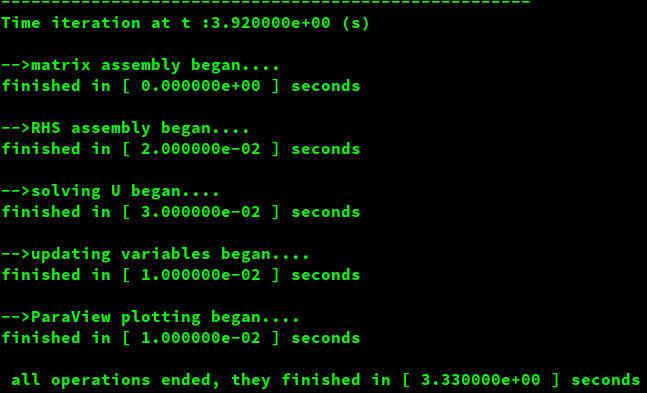
\includegraphics[width=0.4\textwidth]{./Images/ed-time-seq.png}
\caption{Time logging output produced for parallel run on 2 processes.\label{time-seq-ed}}
\end{figure}
